%----------------------------------------------------------------------------------------
%	PACKAGES AND OTHER DOCUMENT CONFIGURATIONS
%----------------------------------------------------------------------------------------
\documentclass[a4paper,11pt]{article}
\usepackage[a4paper,textwidth=140mm,textheight=245mm]{geometry}
\usepackage[utf8]{inputenc}
\usepackage{listings}
\usepackage{graphicx}
\usepackage{mathtools}
\usepackage{subscript}
\makeatletter
\renewcommand{\section}{\@startsection
   {section}%                         name
   {1}%                               level
   {0mm}%                             indent
   {-1.5\baselineskip}%               space above header
   {0.5\baselineskip}%                space under header
   {\sffamily\bfseries\upshape\normalsize}}% style
\renewcommand{\subsection}{\@startsection
   {subsection}%                      name
   {2}%                               level
   {0mm}%                             indent
   {-0.75\baselineskip}%              space above header
   {0.25\baselineskip}%               space under header
   {\rmfamily\normalfont\slshape\normalsize}}% style
\renewcommand{\subsubsection}{\@startsection
   {subsubsection}%                    name
   {3}%                               level
   {-10mm}%                             indent
   {-0.75\baselineskip}%              space above header
   {0.25\baselineskip}%               space under header
   {\rmfamily\normalfont\slshape\normalsize}}% style
\makeatother
\begin{document}

\begin{titlepage}
\title{TATA57 Summary:}
\author{Martin Söderén\\ marso329@student.liu.se\\900929-1098}
\date{\today}
\maketitle
\vfill % Fill the rest of the page with whitespace
\thispagestyle{empty}
\end{titlepage}

\section{general}
Difference equation--Z-transform \newline
differental equation with initial conditions-laplace-transform \newline
differental equation without initial conditions-fourier-transform
differental equation without initial conditions and the solutions has a period of 2*pi-- fourier series on comples form
%Fourier series real form
\section{Fourier series(real form)}
$$F(x)=\dfrac{a_0}{2}+\sum_{k=1}^{\infty}(a_k*cos(k*x)+b_k*sin(k*x))$$
Where:
$$a_k=\dfrac{1}{\pi}\int_{-\pi}^{\pi}f(x)*cos(k*x)dx$$
$$b_k=\dfrac{1}{\pi}\int_{-\pi}^{\pi}f(x)*sin(k*x)dx$$
Where:
	$$f(x)\; has\;a\;period \; of \; 2 \pi$$
Note that b\textsubscript{0}=0
$$\lim_{k \to \infty} F(x) = f(x)$$
\subsection{general}
Describes a periodic function as a sum of sinus function.
\newline
\centerline{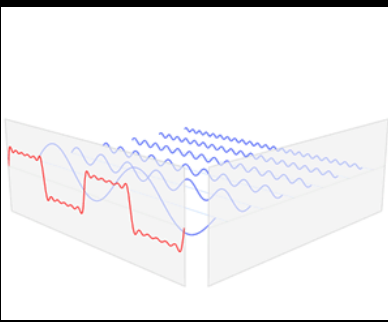
\includegraphics[scale=0.6]{fseries}}
\subsection{example}
\[ f(t) = \left\{
  \begin{array}{l l}
    0 & \quad -\pi \; \leq t<0\\
    1 & \quad 0\leq t<\pi 
  \end{array} \right.\]
  $$f(t) \;has\;a\;period\;of\;2\pi$$
Problems:
\begin{enumerate}
\item calculate Fourier series
\item calculate which values the series converges to at a t=0,-pi,pi
\item calculate the value of the series:$$\sum_{n=1}^{\infty}\dfrac{1}{(2n-1)^2}$$

\end{enumerate}
\subsubsection{1:}
begin with calculating a0
$$a_0=\dfrac{1}{\pi}\int_{0}^{\pi}f(t)dt=\dfrac{1}{\pi}\int_{0}^{\pi}1dx=\dfrac{1}{\pi}\pi=1$$
now the coefficients
$$a_n=\dfrac{1}{\pi}\int_{-\pi}^{\pi}f(x)cos(nx)dx=\dfrac{1}{\pi}\int_{0}^{\pi}cos(nx)dx=\dfrac{1}{\pi}\left(\dfrac{sin(nt)}{n}\right)_{0}^{\pi}=\dfrac{1}{\pi n}0=0$$

$$b_n=\dfrac{1}{\pi}\int_{-\pi}^{\pi}f(x)sin(nx)dx=\dfrac{1}{\pi}\int_{0}^{\pi}sin(nx)dx=\dfrac{1}{\pi}\left(\dfrac{-cos(nt)}{n}\right)_{0}^{\pi}=-\dfrac{1}{\pi n}(cos(\pi n)-cos(0))=$$
$$\dfrac{1-cos(\pi n)}{\pi n}$$
which can be rewritten to:
$$\dfrac{1}{\pi}\dfrac{2}{2n-1}$$
put this in the definition of Fourier transform and you get:
$$f(t)=\dfrac{1}{2}+\dfrac{2}{\pi}\sum_{n=1}^{\infty}\dfrac{1}{2n-1}sin(nt)$$

\subsection{2:}
f(t) satifies dirischlets conditions so the series converges towards:
$$\dfrac{f(t_+)+f(t_-)}{2}$$ 
this gives that:
$$at \; t=0,\pi,-\pi$$
the series converges towards 1/2 since in all those points the functions switches between 0 and 1
\subsection{3:}
By using the less general case of parseval theorem we get:
$$\dfrac{1}{\pi}\int_{0}^{\pi}|1|^2dt=\dfrac{1}{2}+\dfrac{4}{\pi^2}\sum_{n=1}^{\infty}(\dfrac{1}{(2n-1)^2})$$
which gives:
$$\sum_{n=1}^{\infty}(\dfrac{1}{(2n-1)^2})=\dfrac{\pi^2}{8}$$

%Fourier series complex form
\section{Fourier series(complex form)}
$$F(x)=\sum_{-\infty}^{\infty}C_k*e^{ikx}$$
$$C_k=\dfrac{1}{2\pi}\int_{-\pi}^{\pi}f(x)e^{-ikx}dx$$
Where:
	$$f(x)\; has\;a\;period \; of \; 2 \pi$$
\subsection{General}
As real form
\subsection{Example:}
solve:
$$y''(t)-2y(t+\pi)=cos(t)$$
y'' exists so y and y' are continuous
We can change the equation to:
$$y''(t)=2y(t+\pi)+cos(t)$$
from this we can see that y'' is continuous since y and cos are continuous. Because both y and cos are differentiable and their derivatives are continuous then y'' is differentiable and continuous.
Now we know that y y' and y'' fulfills dirischlets conditions and we can put them equal their fourier series.
We use the complex form:
$$y=\sum_{-\infty}^{\infty}C_ke^{ikt}$$
$$y'=\sum_{-\infty}^{\infty}ikC_ke^{ikt}$$
$$y''=\sum_{-\infty}^{\infty}(ik)^2C_ke^{ikt}$$
$$y(t+\pi)=\sum_{-\infty}^{\infty}C_ke^{ik(t+\pi)}$$
$$y(t+\pi)=\sum_{-\infty}^{\infty}(-1)^k*C_ke^{ik(t)}$$
cos in complex form:
$$cos(t)=\dfrac{e^{it}}{2}+\dfrac{e^{-it}}{2}$$
this gives the equation:
$$\sum_{-\infty}^{\infty}(ik)^2C_ke^{ikt}-2*\sum_{-\infty}^{\infty}(-1)^k*C_ke^{ik(t)}=\dfrac{e^{it}}{2}+\dfrac{e^{-it}}{2}$$
$$\sum_{-\infty}^{\infty}((ik)^2-2(-1)^k)*C_ke^{ikt}=\dfrac{e^{it}}{2}+\dfrac{e^{-it}}{2}$$
from this you can see that:
$$(ik)^2-2(-1)^k=0 \;for\; k\neq \pm 1$$
This has no integer solution so :
$$C_k=0 \; for \; k\pm1$$
solutions for:
$$k\pm1$$

gives:
$$C_1=1/2\; and\; C_{-1}=1/2$$
combined with:
$$y=\sum_{-\infty}^{\infty}C_ke^{ikt}$$
gives:
$$y(t)=cos(t)$$

\section{example 2}
Determine all solutions to :
$$y'(t)+y(t+\pi)=cos(t)+sin(2t) \;which \;are\;2\pi \;periodic $$
y(t) is continuous since y'(t) exists for all t. y'(t) is continuous since it is the differnce between two continuous functions. In the same way it follows that y''(t) exists and is continuous. Thuse we can set(from example 1):
$$y'=\sum_{-\infty}^{\infty}ikC_ke^{ikt}$$
$$y(t+\pi)=\sum_{-\infty}^{\infty}C_ke^{ik(t+\pi)}$$
$$cos(t)=\dfrac{e^{it}}{2}+\dfrac{e^{-it}}{2}$$
$$sin(t2)=\dfrac{e^{i2t}}{2i}-\dfrac{e^{-i2t}}{2i}$$
put all this in the equation:
$$\sum_{-\infty}^{\infty}ikC_ke^{ikt}+\sum_{-\infty}^{\infty}C_ke^{ik(t+\pi)}=\dfrac{e^{it}}{2}+\dfrac{e^{-it}}{2}+\dfrac{e^{i2t}}{2i}-\dfrac{e^{-i2t}}{2i}$$
$$\rightarrow$$
$$\sum_{-\infty}^{\infty}C_ke^{ikt}(ik+(-1)^k)=\dfrac{e^{it}}{2}+\dfrac{e^{-it}}{2}+\dfrac{e^{i2t}}{2i}-\dfrac{e^{-i2t}}{2i}$$
this gives :
$$(ik+(-1)^k)C_k=0 \;for\; k\ne\pm1,\pm2$$
$$\rightarrow$$
$$C_k=0 \;for \;k\ne\pm1,\pm2$$
$$(i-1)C_1=\dfrac{1}{2}$$
$$C_1=-\dfrac{1}{2-2i}=-\dfrac{(2+2i)}{(2-2i)(2+2i)}=-\dfrac{(1+i)}{4}$$
the same calculations for c=-1,2,-2 gives:
$$c_{-1}=-\dfrac{(1-i)}{4}$$
$$c_{2}=-\dfrac{(2+i)}{10}$$
$$c_{-2}=-\dfrac{(2-i)}{10}$$
put this in the definition of Fourier series gives:
$$f(t)=-\dfrac{(1+i)}{4}e^{it}-\dfrac{(1-i)}{4}e^{-it}-\dfrac{(2+i)}{10}e^{i2t}-\dfrac{(2-i)}{10}e^{-i2t}$$
which can be rewitten to:
$$f(t)=\dfrac{1}{2}(sin(t)-cos(t))+\dfrac{1}{5}(sin(2t)-2cos(2t))$$



%fourier transform
\section{Fourier Transform}
$$F(W)=\int_{-\infty}^{\infty} f(t)e^{-iwt}dt$$
\subsection{General}
Describes a function in the frequence-domain
\subsection{example}
Solve:
$$y'(t)+\int_{-\infty}^{\infty}y(t-u)e^{-u}\chi(u)du=e^{-t}\chi(t)$$
$$F[y'(t)]=i\omega Y(\omega)$$
important rule:
$$F[\int_{-\infty}^{\infty}y(t-u)g(u)du]=Y(\omega)G(\omega)$$
with 
$$g(u)=e^{-u}\chi(u)$$
$$F[\int_{-\infty}^{\infty}y(t-u)e^{-u}\chi(u)du]=Y(\omega)\dfrac{1}{1+i\omega}$$
and
$$F[e^{-t}\chi(t)]=\dfrac{1}{1+i\omega}$$
put all this in the equation:
$$Y(\omega)(i\omega+\dfrac{1}{1+i\omega})=\dfrac{1}{1+i\omega}$$
$$\rightarrow$$
$$Y(\omega)=\dfrac{1}{(i\omega)^2+i\omega+1}$$
By completing the square we get
$$Y(\omega)=\dfrac{1}{(\dfrac{1}{2}+\dfrac{i\sqrt{3}}{2}+i\omega)(\dfrac{1}{2}-\dfrac{i\sqrt{3}}{2}+i\omega)}$$
$$=\dfrac{A}{\dfrac{1}{2}+\dfrac{i\sqrt{3}}{2}+i\omega}+\dfrac{B}{\dfrac{1}{2}-\dfrac{i\sqrt{3}}{2}+i\omega}$$
A and B can have both real and imaginary parts
$$=\dfrac{A(\dfrac{1}{2}-\dfrac{i\sqrt{3}}{2}+i\omega)+B(\dfrac{1}{2}+\dfrac{i\sqrt{3}}{2}+i\omega)}{(\dfrac{1}{2}+\dfrac{i\sqrt{3}}{2}+i\omega)(\dfrac{1}{2}-\dfrac{i\sqrt{3}}{2}+i\omega)}$$
Finding good values for A and B can be tricky. But in this case you can test with only real parts and then you can see that 
A=-B to get rid of the frequence parts and then you also get rid of the constant real part and you are left with the imaginary part which can be removed with a constant.
With A=1 and B=-1:
$$\dfrac{-\dfrac{i\sqrt{3}}{2}-\dfrac{i\sqrt{3}}{2}}{(\dfrac{1}{2}+\dfrac{i\sqrt{3}}{2}+i\omega)(\dfrac{1}{2}-\dfrac{i\sqrt{3}}{2}+i\omega)}$$
we want 1 in the numerator:
$$-\dfrac{1}{i\sqrt{3}}\dfrac{-i\sqrt{3}}{(\dfrac{1}{2}+\dfrac{i\sqrt{3}}{2}+i\omega)(\dfrac{1}{2}-\dfrac{i\sqrt{3}}{2}+i\omega)}=Y(\omega)$$
this gives:
$$Y(\omega)=\dfrac{1}{i\sqrt{3}}(\dfrac{1}{\dfrac{1}{2}+i(\omega-\dfrac{\sqrt{3}}{2})}-\dfrac{1}{\dfrac{1}{2}+i(\omega+\dfrac{\sqrt{3}}{2})})$$
$$F[\dfrac{1}{i\omega+\dfrac{1}{2}}]=e^{-\dfrac{t}{2}}\chi(t)$$
important rule:
$$F[e^{iat}f(t)]=F(\omega -a)$$
$$F[\dfrac{1}{i(\omega-\dfrac{\sqrt{3}}{2})+\dfrac{1}{2}}]=e^{i\dfrac{\sqrt{3}}{2}t}e^{-\dfrac{t}{2}}\chi(t)$$
and
$$F[\dfrac{1}{i(\omega+\dfrac{\sqrt{3}}{2})+\dfrac{1}{2}}]=e^{-i\dfrac{\sqrt{3}}{2}t}e^{-\dfrac{t}{2}}\chi(t)$$
$$y(t)=\dfrac{1}{i\sqrt{3}}(e^{i\dfrac{\sqrt{3}}{2}t}e^{-\dfrac{t}{2}}\chi(t)-e^{-i\dfrac{\sqrt{3}}{2}t}e^{-\dfrac{t}{2}}\chi(t))=$$
$$y(t)=\dfrac{1}{i\sqrt{3}}(e^{i\dfrac{\sqrt{3}}{2}t}-e^{-i\dfrac{\sqrt{3}}{2}t})e^{-\dfrac{t}{2}}\chi(t)=$$
$$y(t)=\dfrac{2}{\sqrt{3}}(sin(t\dfrac{\sqrt{3}}{2}))e^{-\dfrac{t}{2}}\chi(t)$$
%Laplace transform
\section{Laplace tranform}
$$F(s)=\int_{0}^{\infty}f(t)e^{-st}dt$$
If f is a periodic function with period T:
$$F(s)=\dfrac{1}{1-e^{-sT}}\int_{0}^{T}f(t)e^{-st}dt$$
\subsection{general}
Describes a function in the frequence-domain but compared to Fourier transform which is a superposition of sinusoids its a superposition of moments.
Good for solving linear differential equations with inital values or boundary values. For example control engieering problems.
\subsection{good to remember}
\[  \left\{
  \begin{array}{l l}
    sin(t) & \quad 0 \; \leq t<\pi\\
    0 & \quad \pi \leq t 
  \end{array} \right.\]
  can be written as:
  $$sin(t)\chi(t)+sin(t-\pi)\chi(t-\pi)$$
  
\subsection{example}
solve
$$x''(t)+4x'(t)+4x(t)=\chi(t-1)[cos(t-1)+2sin(t-1)]$$
for
$$t\geq0,x(0)=1,x'(0)=0$$
tranformation:
$$x''(t)=s^2F(s)-sf(0)-f'(0)=s^2F(s)-s$$
$$x'(t)=sF(s)-f(0)=sF(s)-1$$
$$x(t)=F(s)$$
$$\chi(t-1)cos(t-1)=e^{-s}\dfrac{s}{s^2+1}$$
$$2*\chi(t-1)sin(t-1)=2e^{-s}\dfrac{1}{s^2+1}$$
put all this in the equation gives
$$s^2F(s)-s+4(sF(s)-1)+4F(s)=e^{-s}\dfrac{s}{s^2+1}+e^{-s}\dfrac{2}{s^2+1}$$
$$\rightarrow F(s)(s^2+4s+4)=e^{-s}\dfrac{s+2}{s^2+1}+s+4$$
$$F(s)=e^{-s}\dfrac{1}{(s^2+1)(s+2)}+\dfrac{s+4}{(s+2)^2}$$
$$\dfrac{s+4}{(s+2)^2}=\dfrac{s+2+2}{(s+2)^2}=\dfrac{s+2}{(s+2)^2}+\dfrac{2}{(s+2)^2}=\dfrac{1}{s+2}+\dfrac{2}{(s+2)^2}$$
$$\dfrac{1}{(s^2+1)(s+2)}=\dfrac{As+B}{s^2+1}+\dfrac{C}{s+2}=\dfrac{(As+B)(s+2)}{(s^2+1)(s+2)}+\dfrac{C(s^2+1)}{(s+2)(s^2+1)}=\dfrac{(As+B)(s+2)+C(s^2+1)}{(s+2)(s^2+1)}$$
$$(As+B)(s+2)+C(s^2+1)=As^2+2As+Bs+2B+Cs^2+C$$
This gives the equationsystem:
$$A+C=0,2A+B=0,2B+C=1$$
which can be solved using linear algebra:\newline
$ \begin{vmatrix} 1&0&1&0\\ 2&1&0&0\\0&2&1&1 \end{vmatrix}$=
$ \begin{vmatrix} 1&0&1&0\\ 0&1&-2&0\\0&2&1&1 \end{vmatrix}$=
$ \begin{vmatrix} 1&0&1&0\\ 0&1&-2&0\\0&0&1&1/5 \end{vmatrix}$=
$ \begin{vmatrix} 1&0&0&-1/5\\ 0&1&0&2/5\\0&0&1&1/5 \end{vmatrix}$
$$\dfrac{1}{(s^2+1)(s+2)}=\dfrac{As+B}{s^2+1}+\dfrac{C}{s+2}=-\dfrac{1}{5}\dfrac{s-2}{s^2+1}+\dfrac{1}{5}\dfrac{1}{s+2}$$
this gives:
$$F(s)=\dfrac{e^{-s}}{5}(\dfrac{1}{s+2}-\dfrac{s-2}{s^2+1})+\dfrac{1}{s+2}+\dfrac{2}{(s+2)^2}$$
$$\dfrac{1}{s+2}=L[e^{-2t}]$$
$$-\dfrac{s}{s^2+1}=L[-cos(t)]$$
$$-\dfrac{2}{s^2+1}=L[-2sin(t)]$$
$$\dfrac{2}{(s+2)^2}=L[2te^{-2t}]$$
important rule:
$$L[\chi(t-a)f(t-a)]=e^{-as}F(s)$$
$$\dfrac{e^{-s}}{5}\dfrac{1}{s+2}=L[\dfrac{1}{5}\chi(t-1)e^{-2(t-1)}]$$
$$-\dfrac{e^{-s}}{5}\dfrac{s}{s^2+1}=L[-\dfrac{1}{5}\chi(t-1)cos(t-1)]$$
$$\dfrac{2e^{-s}}{5}\dfrac{1}{s^2+1}=L[-\dfrac{2}{5}\chi(t-1)sin(t-1)]$$
this gives:
$$x(t)=\dfrac{1}{5}\chi(t-1)e^{-2(t-1)}-\dfrac{1}{5}\chi(t-1)cos(t-1)+\dfrac{2}{5}\chi(t-1)sin(t-1)+e^{-2t}+2te^{-2t}$$
$$x(t)=\dfrac{1}{5}\chi(t-1)(e^{-2(t-1)}-cos(t-1)+2sin(t-1))+e^{-2t}(1+2t)$$
%Z-transform
\section{Z-transform}
$$Z[f(k)]=\sum_{k=0}^{\infty}\dfrac{f(k)}{z^k}$$
\subsection{general}
Transforms a discrete-time signal into the complex frequency domain
Good for solving difference equations. For example:
$$f(k+1)=f(k)+1$$
\subsection{Example}
solve:
$$y(k+2)-5y(k+1)+6y(k)=2^k\;k=0,1,,,,,,$$
Where:
$$y(0)=y(1)=0$$
$$y(k+2)=z^2F(z)-z^2f(0)-zf(1)$$
$$y(k+1)=zF(z)-zf(0)$$
$$y(k)=F(z)$$
Which with the inital bounds gives:
$$y(k+2)=z^2F(z)$$
$$y(k+1)=zF(z)$$
$$y(k)=F(z)$$
and
$$2^k=\dfrac{z}{z-2}$$
put all this into the equation gives:
$$z^2F(z)-5zF(z)+6F(z)=\dfrac{z}{z-2}$$
$$F(z)=\dfrac{z}{(z-2)(z^2-5z+6)}$$
$$F(z)=\dfrac{z}{(z-2)(z-2)(z-3)}$$
$$\dfrac{F(z)}{z}=\dfrac{1}{(z-2)^2(z-3)}$$
We want to split the denominator up:
$$\dfrac{1}{(z-2)^2(z-3)}=\dfrac{Az+B}{(z-2)^2}+\dfrac{C}{z-3}=\dfrac{(Az+B)(z-3)+c(z-2)^2}{(z-2)^2(z-3)}$$
$$=\dfrac{Az^2-3Az+Bz-3B+Cz^2+C4-4Cz}{(z-2)^2(z-3)}$$
Which gives the equation system:
$$A+C=0 \;-3A+B-4C=0 \; -3B+4C=1$$
which can be solved using linear algebra:\newline
$ \begin{vmatrix} 1&0&1&0\\ -3&1&-4&0\\0&-3&4&1 \end{vmatrix}$
=
$ \begin{vmatrix} 1&0&1&0\\ 0&1&-1&0\\0&-3&4&1 \end{vmatrix}$=
$ \begin{vmatrix} 1&0&1&0\\ 0&1&-1&0\\0&0&1&1 \end{vmatrix}$=
$ \begin{vmatrix} 1&0&0&-1\\ 0&1&0&1\\0&0&1&1 \end{vmatrix}$
which gives:
$$-z^2+3z+z-3+z^2+4-4z=1$$
$$F(z)=\dfrac{-z^2}{(z-2)^2}+\dfrac{z}{(z-2)^2}+\dfrac{z}{z-3}$$
which gives
$$f(K)=-(k+1)2^k+\dfrac{1}{2}k2^k+3^k=$$
$$-(\dfrac{1}{2}k+1)2^k+3^k \; for \: k=0,1,2,,,,$$
%Parseval theorem
\section{Parseval theorem}
$$\int_{-\infty}^{\infty}|f(x)|^2dx=\int_{-\infty}^{\infty}|F(x)|^2dx$$
less general:
$$\dfrac{1}{\pi}\int_{-\pi}^{\pi}|f(t)|^2dt=\dfrac{1}{2}a_0^2+\sum_{n=1}^{\infty}(a_n^2+b_n^2)$$

%plancherels thoerem
\section{Plancherels theorem}
$$\int_{-\infty}^{\infty}|f(x)|^2dx=\dfrac{1}{2\pi}\int_{-\infty}^{\infty}|F(\omega)|^2d\omega$$

%dirischlets conditions
\section{Dirichlets conditions}
\begin{itemize}
    \item f(x) must be absolutely integrable over a period.\newline
    \item f(x) must have a finite number of extrema in any given bounded interval, i.e. there must be a finite number of maxima and minima in the interval.\newline
    \item f(x) must have a finite number of discontinuities in any given bounded interval, however the discontinuity cannot be infinite.\newline
    \item f(x) must be bounded
\end{itemize}

%even and odd functions
\section{odd and even functions}
cos(x) is even since
$$cos(-x)=cos(x)$$
sin(x) is odd since
$$sin(-x)=-sin(x)$$
odd*odd=even \newline
even*even=even \newline
odd*even=odd\newline

\end{document}